\documentclass[a4paper,UTF8]{article}
\usepackage{ctex}
\usepackage[margin=1.25in]{geometry}
\usepackage{color}
\usepackage{graphicx}
\usepackage{amssymb}
\usepackage{amsmath}
\usepackage{amsthm}
\usepackage{tcolorbox}
\usepackage{enumerate}
\usepackage{hyperref}
%\usepackage[thmmarks, amsmath, thref]{ntheorem}
\theoremstyle{definition}
\newtheorem*{solution}{Solution}
\newtheorem*{prove}{Proof}
\usepackage{multirow}              
\usepackage{graphicx}
\usepackage{pythonhighlight}
\setlength{\evensidemargin}{.25in}
\setlength{\textwidth}{6in}
\setlength{\topmargin}{-0.5in}
\usepackage{float}
\setlength{\topmargin}{-0.5in}
% \setlength{\textheight}{9.5in}
%%%%%%%%%%%%%%%%%%此处用于设置页眉页脚%%%%%%%%%%%%%%%%%%
\usepackage{fancyhdr}                                
\usepackage{lastpage}                                           
\usepackage{layout}                                             
\footskip = 10pt 
\pagestyle{fancy}                    % 设置页眉                 
\lhead{2020年春季}                    
\chead{机器学习导论}                                                
% \rhead{第\thepage/\pageref{LastPage}页} 
\rhead{作业一}                                                                                               
\cfoot{\thepage}                                                
\renewcommand{\headrulewidth}{1pt}  			%页眉线宽,设为0可以去页眉线
\setlength{\skip\footins}{0.5cm}    			%脚注与正文的距离           
\renewcommand{\footrulewidth}{0pt}  			%页脚线宽,设为0可以去页脚线

\makeatletter 									%设置双线页眉                                        
\def\headrule{{\if@fancyplain\let\headrulewidth\plainheadrulewidth\fi%
		\hrule\@height 1.0pt \@width\headwidth\vskip1pt	%上面线为1pt粗  
		\hrule\@height 0.5pt\@width\headwidth  			%下面0.5pt粗            
		\vskip-2\headrulewidth\vskip-1pt}      			%两条线的距离1pt        
	\vspace{6mm}}     								%双线与下面正文之间的垂直间距              
\makeatother  

%--

%--
\begin{document}
\title{机器学习导论\\习题一}
\author{181220028, 李佩然, 181220028@smail.nju.edu.cn}
\maketitle


\section*{学术诚信}

本课程非常重视学术诚信规范,助教老师和助教同学将不遗余力地维护作业中的学术诚信规范的建立。希望所有选课学生能够对此予以重视。\footnote{参考尹一通老师\href{http://tcs.nju.edu.cn/wiki/}{高级算法课程}中对学术诚信的说明。}

\begin{tcolorbox}
	\begin{enumerate}
		\item[(1)] 允许同学之间的相互讨论,但是{\color{red}\textbf{署你名字的工作必须由你完成}},不允许直接照搬任何已有的材料,必须独立完成作业的书写过程;
		\item[(2)] 在完成作业过程中,对他人工作(出版物、互联网资料)中文本的直接照搬(包括原文的直接复制粘贴及语句的简单修改等)都将视为剽窃,剽窃者成绩将被取消。{\color{red}\textbf{对于完成作业中有关键作用的公开资料,应予以明显引用}};
		\item[(3)] 如果发现作业之间高度相似将被判定为互相抄袭行为,{\color{red}\textbf{抄袭和被抄袭双方的成绩都将被取消}}。因此请主动防止自己的作业被他人抄袭。
	\end{enumerate}
\end{tcolorbox}

\section*{作业提交注意事项}
\begin{tcolorbox}
	\begin{enumerate}
		\item[(1)] 请在LaTeX模板中第一页填写个人的姓名、学号、邮箱信息;
		\item[(2)] 本次作业需提交该pdf文件、问题2问题4可直接运行的源码(两个.py文件)、作业2用到的数据文件 (为了保证问题2代码可以运行),将以上四个文件压缩成zip文件后上传,例如181221001.zip;
		\item[(3)] 未按照要求提交作业,或提交作业格式不正确,将会被扣除部分作业分数;
		\item[(4)] 本次作业提交截止时间为3月15日23:59:59。除非有特殊情况(如因病缓交),否则截止时间后不接收作业,本次作业记零分。
	\end{enumerate}
\end{tcolorbox}

\newpage
\section*{Problem 1}
若数据包含噪声,则假设空间中有可能不存在与所有训练样本都一致的假设,此时的版本空间是什么?在此情形下,试设计一种归纳偏好用于假设选择。
\begin{solution}
\phantom{abc}

根据教材定义,存在多个与所有训练样本一致时,版本空间为“与训练集一致的‘假设集合’”。
那么存在噪声时,可以将“与训练集一致”的条件适当放宽为“与训练集大部分样例一致(如95\%)” 。不选择与最多样本一致的原因是,考虑噪声的情况下,与最多样本一致可能会涉及部分噪声点,造成过拟合。

归纳偏好:减少不符合模型的样例个数和与特征和。

~\\
~\\
\end{solution}

\section*{Problem 2 [编程]} 
现有500个测试样例,其对应的真实标记和学习器的输出值如表\ref{table:roc}所示 (完整数据见data.csv文件)。该任务是一个二分类任务,1表示正例,0表示负例。学习器的输出越接近1表明学习器认为该样例越可能是正例,越接近0表明学习器认为该样例越可能是负例。
\begin{table}[!h]
	\centering
	\caption{测试样例表} \vspace{2mm}\label{table:roc}
	\begin{tabular}{c|c c c c c c c c c c c}\hline
		样本 & $x_1$ & $x_2$ & $x_3$  & $x_4$  & $x_5$&...& $x_{496}$& $x_{497}$ & $x_{498}$ & $x_{499}$ & $x_{500}$ \\
		\hline
		标记 & 1  & 1 &  0 &  0  & 0 &... &0& 1 & 0 & 1 & 1\\
		\hline
		输出值 & 0.206  & 0.662 &  0.219 &  0.126  & 0.450 & ... & 0.184&0.505 & 0.445 & 0.994 & 0.602\\
		\hline
	\end{tabular}
\end{table}
\begin{enumerate}[ {(}1{)}]
\item 请编程绘制P-R曲线
\item 请编程绘制ROC曲线,并计算AUC
\end{enumerate}
本题需结合关键代码说明思路,并贴上最终绘制的曲线。建议使用Python语言编程实现。(预计代码行数小于100行)

提示:
\begin{itemize}
	\item 需要注意数据中存在输出值相同的样例。
	\item 
	在Python中,数值计算通常使用Numpy, 表格数据操作通常使用Pandas, 画图可以使用Matplotlib (Seaborn), 同学们可以通过上网查找相关资料学习使用这些工具。未来同学们会接触到更多的Python扩展库,如集成了众多机器学习方法的Sklearn, 深度学习工具包Tensorflow, Pytorch等。
\end{itemize}
\begin{solution}
	\phantom{abc}
\begin{enumerate}[ {(}1{)}]
	\item 以下是计算部分的主体代码:
	\begin{python}
from matplotlib import pyplot as plt
import pandas as pd

dataset = pd.read_csv("./data.csv")
Pre = list()
Rec = list()
TPR = list()
FPR = list()
for i in range(len(dataset)):
	bar = dataset.loc[i, 'output']
	dataset['Prediction'] = dataset.apply(lambda x: 1 if x['output'] >= bar else 0, axis=1)
	dataset['Type'] = dataset.apply(lambda x: True if x['label'] == x['Prediction'] else False, axis=1)
	dataset['TP'] = dataset.apply(lambda x: 1 if x['Type'] is True and x['Prediction'] == 1 else 0, axis=1)
	dataset['FP'] = dataset.apply(lambda x: 1 if x['Type'] is False and x['Prediction'] == 1 else 0, axis=1)
	dataset['TN'] = dataset.apply(lambda x: 1 if x['Type'] is True and x['Prediction'] == 0 else 0, axis=1)
	dataset['FN'] = dataset.apply(lambda x: 1 if x['Type'] is False and x['Prediction'] == 0 else 0, axis=1)

	TP = sum(dataset['TP'])
	FP = sum(dataset['FP'])
	TN = sum(dataset['TN'])
	FN = sum(dataset['FN'])

Pre.append(TP / (TP + FP))
Rec.append(TP / (TP + FN))
TPR.append(TP / (TP + FN))
FPR.append(FP / (TN + FP))
	\end{python}
算法主体思路为遍历每一个可采用的阈值,将其作为分类器的标准,通过DataFrame的apply函数,高效地应用到每一个样例上,然后统计TP、FP、TN、FN。此后在绘制图时,直接使用对应公式生成横纵坐标数组,绘制折线图即可。图\ref{prcurve}为绘制的P-R曲线。
\begin{figure}[H]
	
	\centering
	
	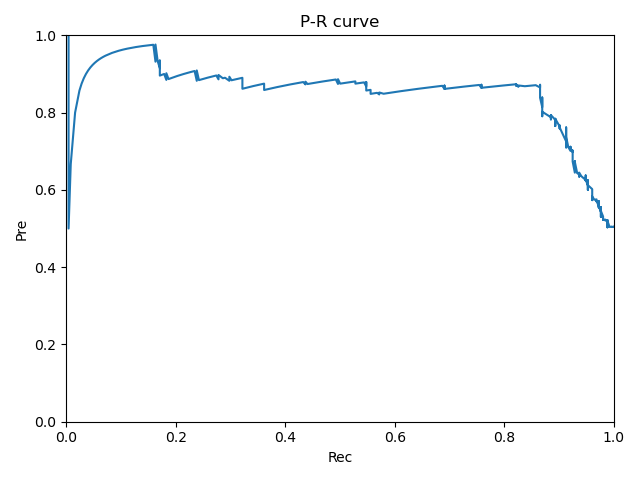
\includegraphics[scale=0.3]{myplot1.png}
	
	\caption{P-R曲线图}
	
\end{figure}\label{prcurve}
	\item
	由于计算的时候将所有可能的$TP, FP, TN, FN$都已经计算出来了,此问中利用公式$TPR=\frac{TP}{TP+FN}$与$FPR = \frac{FP}{TN+FP}$绘图即可,$AUC \approx 0.873$。图\ref{roc}为绘制的ROC曲线图,绿色部分的面积即为AUC。
\begin{figure}[H]
	
	\centering
	
	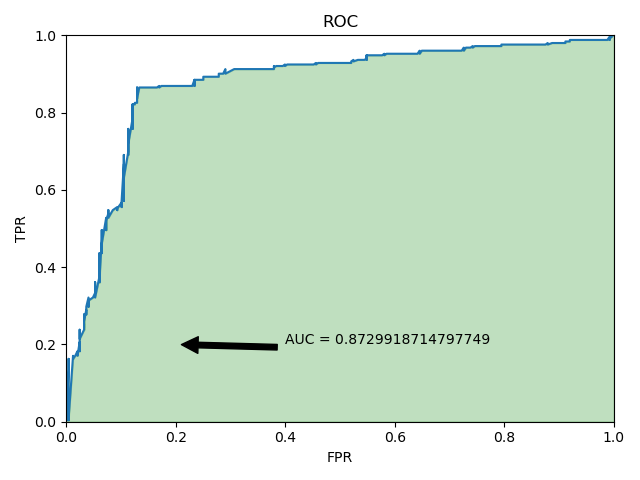
\includegraphics[scale=0.3]{myplot2.png}
	
	\caption{ROC曲线图}
	
\end{figure}\label{roc}

\end{enumerate}

\end{solution}

\section*{Problem 3}
对于有限样例,请证明
\[
\text{AUC} = \frac{1}{m^+m^-}\sum_{x^+\in D^+}\sum_{x^-\in D^-}\left(\mathbb{I}(f(x^+)>f(x^-))+\frac{1}{2}\mathbb{I}(f(x^+)=f(x^-))\right)
\]

\begin{prove}
\phantom{abc}

我们将所有样本点按照预测值从大到小排序,则当阈值从1到0过渡的时候,这些点会依次序从左到右的落在ROC图像上。先不考虑不同类预测值相同的情形以便简化处理。

曲线的起点是点$(0, 0)$,当一个新的点引入曲线时,对应的即是一次阈值的下降。那么,由TPR和FPR的定义我们知道,如果这个点是正例,则曲线端点$y$坐标上升$\frac{1}{m^+}$,如果一个点是负例,则曲线端点$x$坐标右移$\frac{1}{m^-}$,前者不增加与$x$轴围成的面积而后者增加$y\Delta x$的面积。那么我们知道,只有当增加负例的时候增加面积,而增加面积的大小取决于之前的正例数量,增加的面积大小即为$y*\Delta x = \frac{\text{TP}}{\text{TP}+\text{FN}} * \frac{1}{m^-} = \frac{\text{TP}}{m^+m^-}$,而在这个时候的TP就是之前被选到的点数,也就是依据一开始的定义,就是比现在这个负例预测值大的点数,即$\sum_{x^+\in D^+}(\mathbb{I}(f(x^+)>f(x^-))$,所以此时$\text{AUC} = \frac{1}{m^+m^-}\sum_{x^+\in D^+}\sum_{x^-\in D^-}\left(\mathbb{I}(f(x^+)>f(x^-))\right)$

下面考虑不同类预测值相同的情形,但不同类的预测值相同时,加入一个新的点时,如果不会相同则如上述情况,如果与另一类点预测值相同,不妨设有$k_0$个负类,$k_1$个正类,加入这一个点后,横坐标增加了$\frac{k_0}{m^-}$,纵坐标增加了$\frac{k_1}{m^-}$,新增面积是一个梯形,且上底为$\frac{\text{TP}}{\text{TP}+\text{FN}}$,下底为$\frac{\text{TP}}{\text{TP}+\text{FN}}+\frac{k_1}{m^-}$。利用梯形面积公式我们知道,增加的面积为$\frac{\text{TP}}{m^+m^-}+\frac{k}{2(m^+m^-)}$,TP是$\sum_{x^+\in D^+}(\mathbb{I}(f(x^+)>f(x^-))$,而k便是与当前$x^-$相同正例数量,$\sum_{x^+\in D^+}(\mathbb{I}(f(x^+)=f(x^-))$,所以$
\text{AUC} = \frac{1}{m^+m^-}\sum_{x^+\in D^+}\sum_{x^-\in D^-}\left(\mathbb{I}(f(x^+)>f(x^-))+\frac{1}{2}\mathbb{I}(f(x^+)=f(x^-))\right)
$
~\\
~\\
\qed
\end{prove}

\section*{Problem 4 [编程]} 
在数据集$D_1,D_2,D_3,D_4,D_5$运行了$A,B,C,D,E$五种算法,算法比较序值表如表\ref{table:ranking}所示:
\begin{table}[h]
\centering
\caption{算法比较序值表} \vspace{2mm}\label{table:ranking}
\begin{tabular}{c|c c c c c}\hline
数据集 & 算法$A$ & 算法$B$  & 算法$C$  &算法$D$  &算法$E$ \\
\hline
$D_1$ & 2  & 3 &  1 &  5  & 4\\
$D_2$ & 5  & 4 &  2 &  3  & 1\\
$D_3$ & 4  & 5 &  1 &  2  & 3\\
$D_4$ & 2  & 3 &  1 &  5  & 4\\
$D_5$ & 3  & 4 &  1 &  5  & 2\\
\hline
平均序值 & 3.2 &  3.8 & 1.2 &  4 &  2.8 \\
\hline
\end{tabular}
\end{table}

使用Friedman检验$(\alpha=0.05)$判断这些算法是否性能都相同。若不相同,进行Nemenyi后续检验$(\alpha=0.05)$,并说明性能最好的算法与哪些算法有显著差别。本题需编程实现Friedman检验和Nemenyi后续检验。(预计代码行数小于50行)
\begin{solution}
	\phantom{abc}
	
	使用Friedman检验$(\alpha=0.05)$发现$\tau_{\chi^2} \approx 9.92$,$\tau_f \approx 3.94 > 3.007$,所以这些算法的性能并不相同。
	
	使用Nemenyi后续检验$(\alpha=0.05)$发现临界值域$CD=2.728$,经计算可得下表
	\begin{table}[h]
		\centering
		\caption{算法间差别} \vspace{2mm}\label{table:ranking}
		\begin{tabular}{c|c |c| c| c| c}\hline
			有显著差距 & 算法$A$ & 算法$B$  & 算法$C$  &算法$D$  &算法$E$ \\
			\hline
			算法$A$ &   &  &   &    & \\
			\hline
			算法$B$ &   &  &  &    & \\
			\hline
			算法$C$ &   &  &   &  \checkmark  & \\
			\hline
			算法$D$ &   &  & \checkmark  &    & \\
			\hline
			算法$E$ &   &  &   &    & \\
			\hline
		\end{tabular}
	\end{table}
~\\
~\\
\end{solution}
\end{document}